\chapter{Server Security}
\label{chp:bserversec}

In this chapter some thoughts on general basic server security will be given, for security concerning specific programs see the appropriate chapters.

\section{Physical Security}

This section will concern itself with everything except the operating system and installed software that runs under it.

\subsection{Boot Order}
First when we installed ubuntu, we told our BIOS to boot from a CD or USB.  Now if this is the default option all a hacker has to do is insert a live USB or CD and access all your files...  Not cool...

Set the default (and only, if possible) boot media to the hard drive.

\subsection{BIOS password}

There is some debate about how effective these are... Yes its true that you can overcome the password by shorting a jumper on the motherboard or taking out the CMOS battery, but by setting one you'll force an attacker to go through another step to access the BIOS/Computer, possibly putting them off.

So in short, it doesn't hurt to set one.

\subsection{Case security}

To overcome the point that anyone can bypass the password with physical access to the motherboard, we can prevent this.  Most tower cases come with two hoops on the back that line up, put a padlock in them.  That's what those hoops are there for.


\section{Software Hardening}

This section concerns itself with the software that runs under the OS, and the OS itself.

\subsection{Un-necessary software}

If you are running a server that is likely to come under attack (See: any computer that is connected to the internet) do not run anything that doesn't need to be running.  i.e. Don't run an apache instance if you are not going to use it, it could be an access point for an attacker to gain control of your system.

\subsection{root access}

It has been said in this document a few times that you shouldn't really enable the root user, and only use the sudo function instead.

\subsection{Fail2Ban}

\url{fail2ban.org/wiki/index.php/Main_Page}
\url{www.linux-magazine.com/Online/Features/Intrusion-Detection-with-fail2ban}
\url{linuxaria.com/howto/how-to-protect-apache-with-
fail2ban}

Fail2Ban is a brilliant piece of software which will monitor your log files looking for suspicious behaviour, then ban those that exhibit it.  For example with ssh if someone tries ten different usernames with ten different passwords, fail2ban will recognise this and ban the ip adress before they can correctly guess their way in.  The same happens with apache and people looking for \textit{phpmyadmin} etc.

To install type

\begin{lstlisting}
sudo apt-get install fail2ban
\end{lstlisting}

Now we need to set up which services are going to be run, and configure them.  Navigate to $/etc/fail2ban$ then create a new file called $jail.local$.  This will allow any changes we make to be persistent between updates.

Open up $jail.conf$ and look at the services there, to enable them, write the service name and $enabled = true$ in the jail.local file, as below:

\begin{verbatim}
[ssh]
enabled = true
\end{verbatim}

Any other configuration that you may need to do can also be included here, i.e. port numbers, or a different amount of allow retries:

\begin{verbatim}
[ssh]
enabled = true
port = 500
maxretry = 2
\end{verbatim}

In appendix~\ref{app:fail2banLocal} a working $jail.local$ file can be seen.

The keen readers will notice that there is an entry in the example $jail.local$ that does not correspond with any entry in $jail.conf$.  This is a custom entry that corresponds to a new rule that has been placed in the $filter.d$ directory.  This rule is written in regex form and has been included in appendix~\ref{app:fail2banRule}, this rule looks for anyone trying to access a well known apache exploit for example running the phpmyadmin setup script.

%-----------------------------------------------

\section{Monitoring - INCOMPLETE}

\url{http://www.binarytides.com/linux-commands-monitor-network/}

\begin{lstlisting}
sudo apt-get install iftop nethogs bmon vnstat speedometer
\end{lstlisting}

\begin{table}[!th]
\centering
\begin{tabular}{cc}
\hline
Interface Name & Short\\
\hline
Loopback Interface & lo\\
eth0 & Ethernet Interface 1\\
eth1 & Ethernet Interface 2\\
virbr0 & Virtual Bridge\\
wlan0 & Wi-Fi LAN 0\\
\hline
\end{tabular}
\caption{List of interfaces shown in linux}
\label{tab:interface}
\end{table}

\subsection{iftop}

\begin{lstlisting}
sudo iftop -n -i eth0
\end{lstlisting}

\begin{figure}[!th]
\centering
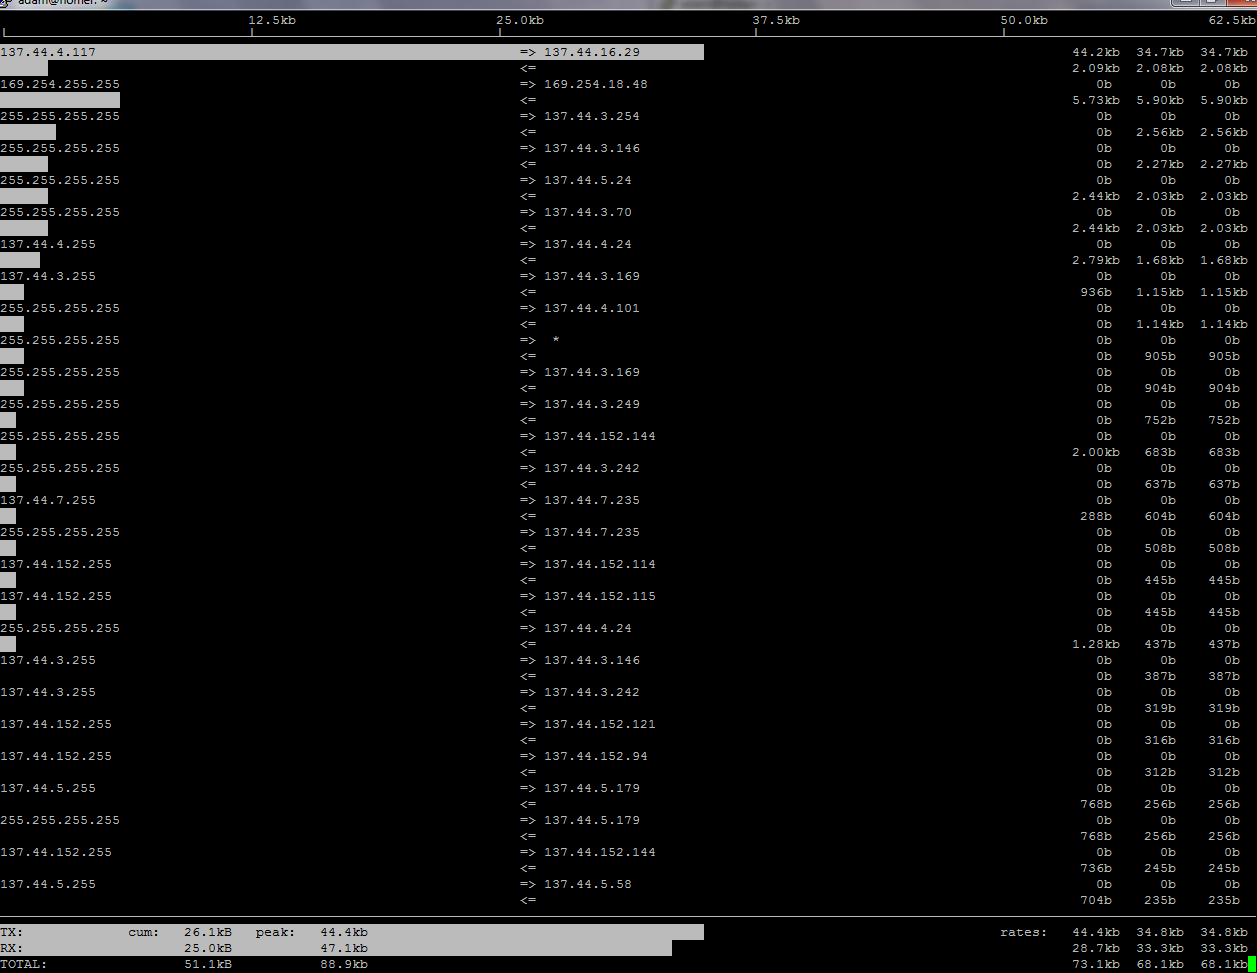
\includegraphics[scale=0.35]{./supportfiles/iftop.png}
\caption{iftop terminal output}
\label{fig:iftop}
\end{figure}

\subsection{nethogs}

\begin{lstlisting}
sudo nethogs
\end{lstlisting}

\begin{figure}[!th]
\centering
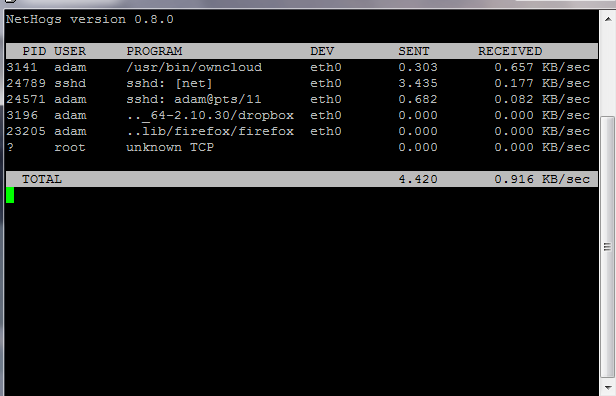
\includegraphics[scale=0.75]{./supportfiles/nethogs.png}
\caption{nethogs terminal output}
\label{fig:nethog}
\end{figure}


\subsection{bmon}

\begin{lstlisting}
bmon
\end{lstlisting}

bmon is used to display graphically the total bps (bytes per second) across all your devices, aswell as in RX (Receiving) and TX (Transmitting) graphs.  See figure~\ref{fig:bmon} for an example of the output, where the interfaces are shown in table\ref{tab:interface}.

\begin{figure}[!th]
\centering
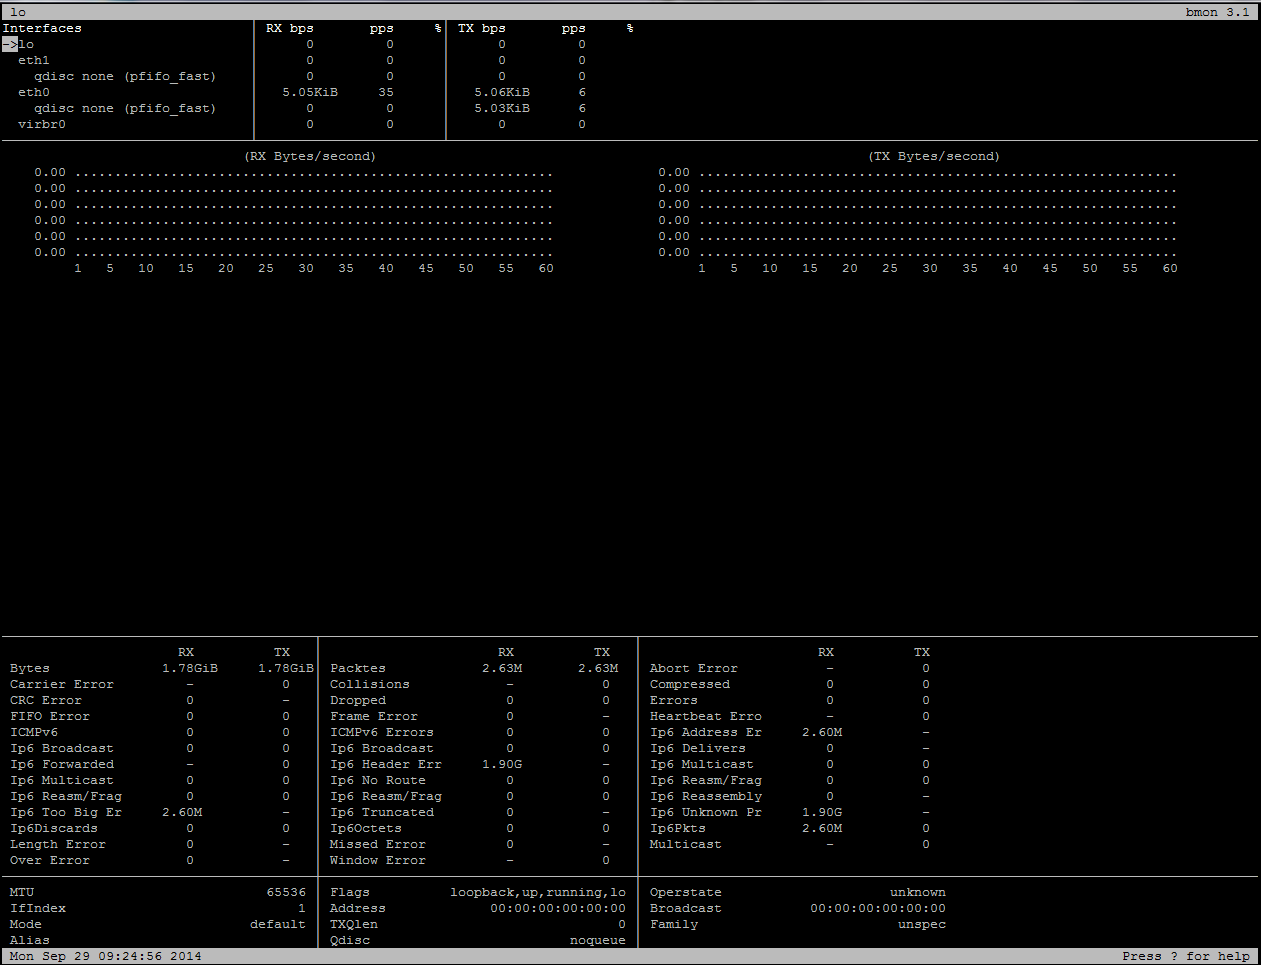
\includegraphics[scale=0.35]{./supportfiles/bmon.png}
\caption{Bmon terminal output}
\label{fig:bmon}
\end{figure}

\subsection{vnstat}

\begin{lstlisting}
sudo vnstat
\end{lstlisting}

\begin{figure}[!th]
\centering
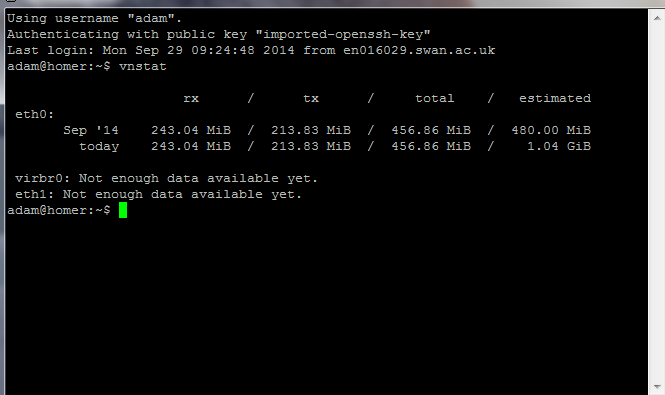
\includegraphics[scale=0.75]{./supportfiles/vnstat.png}
\caption{vnstat terminal output}
\label{fig:vnstat}
\end{figure}

\subsection{speedometer}

\begin{lstlisting}
sudo speedometer -r eth0 -teth0
\end{lstlisting}

\begin{figure}[!th]
\centering
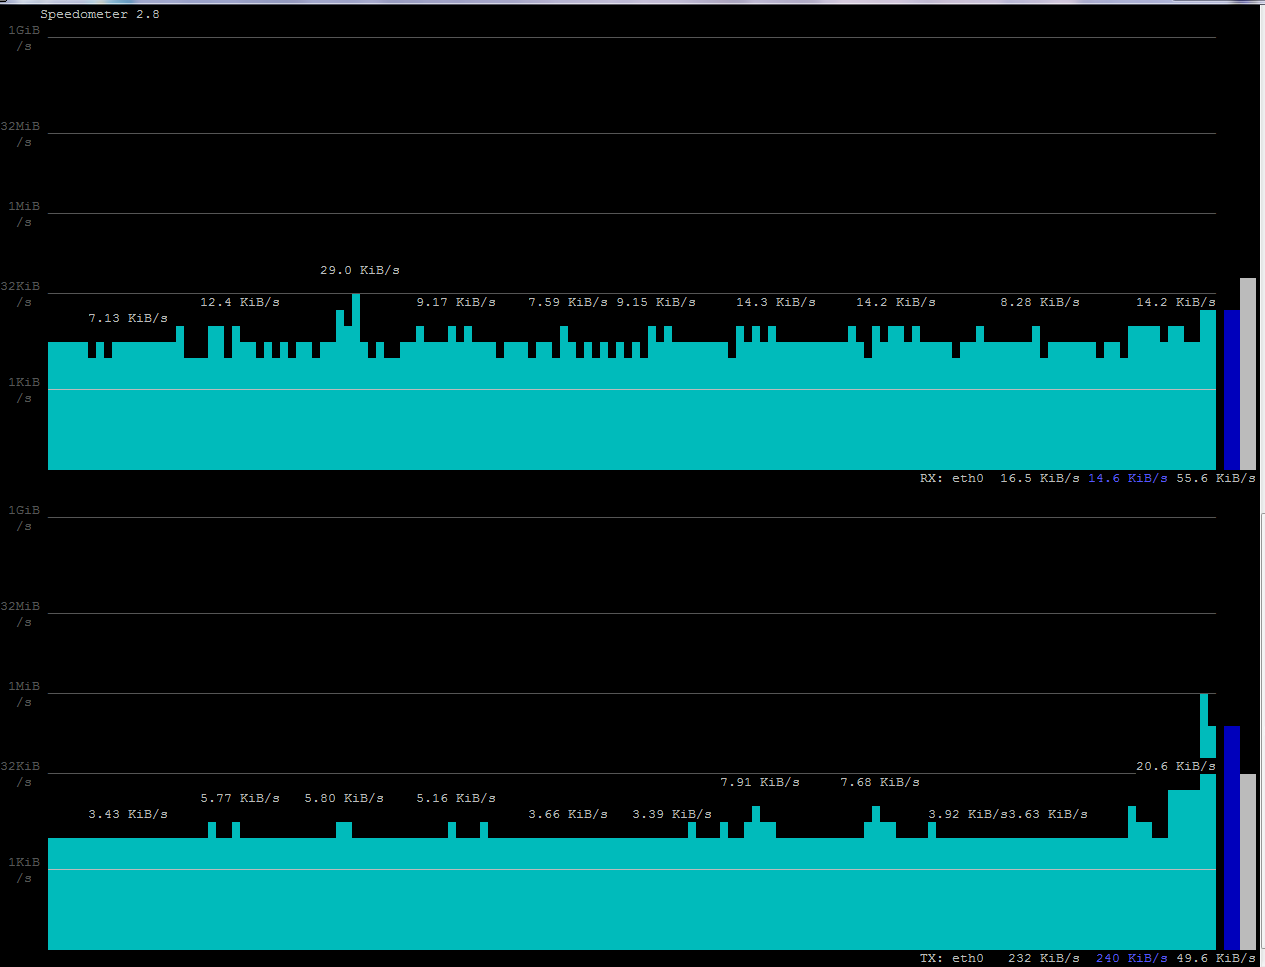
\includegraphics[scale=0.35]{./supportfiles/speedometer.png}
\caption{speedometer terminal output}
\label{fig:speedometer}
\end{figure}


\section{Backup}

Backing up is an important aspect of computer security, if a computer is compromised the best way to overcome it is to start again, see Part~\ref{part:uninstall}.  If this happens, you'll need a backup of all your data to restore.  In this section we see how to generally backup data.

For MySQL we have covered backing up the database into a file in subsection~\ref{ssec:mySQLBackup}.


\section{Monitoring Logs}

Linux systems log everything that happens, the location of these logs can be found in $/var/log/*$.  Table~\ref{tab:logTable} shows the log names and what they contain:

\begin{table}
\centering
\begin{tabular}{cc}
\hline
log name & log description\\
\hline
messages & General log messages\\
boot & System boot log\\
debug & Debugging log messages\\
auth.log & User login and authentication logs\\
deamon.log & Running services such as squid, ntpd, and others log\\
dmesg & Linux kernel ring buffer log\\
dpkg.log & All binary package logs (including installations)\\
faillog & User failed login log (Binary File)\\
karn.log & Kernel log file\\
lpr.log & Printer log file\\
mail & All mail server message log files\\
mysql & MySQL server log file\\
user.log & All userlevel logs\\
xorg.0.log & X.org log\\
apache2/ & Apache web server log files directory\\
lighttpd/ & Lighttpd web server log files directory\\
fsck & fsck command log\\
apport.log & Application crash report + log file\\
\hline
\end{tabular}
\caption{Log Name and Description Table}
\label{tab:logTable}
\end{table}